\section{Preliminares}


\subsection*{Resultados sobre Integração que todos devem saber}
\begin{frame}{Resultados sobre Integração que todos devem saber}
		Seja $(X,\mathcal{M},\mu)$ um espaço de medida
		
		\begin{itemize}
			\item Dizemos que $X$ é \dt{$\sigma$-finito } quando existe uma família enumerável $(X_n)$ em $ \mathcal{M}$ tal que $X=\cup_{n=1}^\infty X_n$ e $\mu(X_n)<+\infty$.
			
			\item Denotaremos por $L^1(X)$ o espaço das \dt{funções integráveis} e definimos
			\[\n{f}_{L^1(X)}=\int_X |f|\,d\mu.\]
			
			\item $f\in L^1(X)$ se, e somente se, $\n{f}_{L^1(X)}<+\infty$.
			
		\end{itemize}
	
	

\end{frame}

\begin{frame}
	\begin{teo}[Teorema da Convergência Dominada de Lebesgue]
		Seja $(f_n)$ uma sequência de funções em $L^1(X)$ que satisfaz:
		\begin{enumerate}[a]
			\item $f_n(x)\to f(x)$ q.s em $X$,
			\item Existe $g\in L^1(X)$ tal que $|f_n(x)|\leq g(x)$ q.s. em $X$.
		\end{enumerate} 
	Então $f\in L^1(X)$ e $\n{f_n-f}_{L^1(X)}\to 0$.
	\end{teo}
\end{frame}

\subsection*{Teorema de Fubini-Tonelli}
\begin{frame}{Teorema de Fubini-Tonelli em \(\R^N\)}
	Sejam $X\subset \R^r$ e $Y\subset \R^s$ conjuntos mensuráveis com \(m_r(X)>0\) e \(m_s(Y)>0\). Então \(X\times Y\subset \R^r\times \R^s\) é mensurável e 
	\[m_{r+s}(X\times Y)=m_r(X)m_s(Y).\]
	
	Além disso, se \(f:X\longrightarrow \bar{\R}\) e \(g:Y\longrightarrow\bar{\R}\) são funções mensuráveis, então a função
	\[h(x,y)=f(x)g(y)\]
	é mensurável.
	 
	



\end{frame}

\begin{frame}{Teorema de Fubini-Tonelli em \(\R^N\)}

	
	Dado $F:X\times Y\longrightarrow \bar{\R}$, definimos as funções
	\[F_x(y)=F(x,y), \ y\in Y \text{ e } F^y(x)=F(x,y),\ x\in X\]
		\begin{teo}[Tonelli]
		Sejam $X\subset \R^r$ e $Y\subset \R^s$ conjuntos mensuráveis.	Se $F:X\times Y\longrightarrow \bar{\R}$ é uma \dt{função mensurável} e {\color{red}não negativa}, então as funções $f(x)=\int_{Y}F_x\,dy$ e $g(y)=\int_{X}F^y\,dx$ são mensuráveis e 
		\begin{equation*}
			\int_{X\times Y}F(x,y) \, dxdy=\int_{X}\left[\int_Y F(x,y)\,dy \right] \,dx=\int_{Y}\left[\int_X F(x,y)\,dx \right] \,dy		
		\end{equation*}
	\end{teo}

\end{frame}

\begin{frame}
%	
\begin{teo}[Fubini]
Sejam $X\subset \R^r$ e $Y\subset \R^s$ conjuntos mensuráveis. Se {\color{red}$F\in L^1(X\times Y)$}, então 
\begin{enumerate}
\item $F_x\in L^1(Y)$ q.t.p.  $x\in X$ e $F^y\in L^1(X)$ q.t.p  $y\in Y$.
\item $f(x)=\int_{Y}F_x\,dy\in L^1(X)$ e $g(y)=\int_{X}F^y\,d\,x\in L^1(Y)$.
			\end{enumerate}	
		Além disso, 
		\begin{equation*}
			\int_{X\times Y}F(x,y) \, dxdy=\int_{X}\left[\int_Y F(x,y)\,dy \right] \,dx=\int_{Y}\left[\int_X F(x,y)\,dx \right] \,dy		
		\end{equation*}
\end{teo}
\end{frame}

%\begin{frame}{Teorema de Fubini-Tonelli}
%	Sejam $(X,\mathcal{M},\mu)$ e $(Y,\mathcal{N},\nu)$ espaços de medida e seja $X\times Y$ munido com a medida produto.
%	 
%	
%	Dado $F:X\times Y\longrightarrow \bar{\R}$, definimos as funções
%	\[F_x(y)=F(x,y), \ y\in Y \text{ e } F^y(x)=F(x,y),\ x\in X\]
%		\begin{teo}[Tonelli]
%		Sejam $(X,\mathcal{M},\mu)$ e $(Y,\mathcal{N},\nu)$ espaços de medida \dt{$\sigma$-finitos}.	Se $F:X\times Y\longrightarrow \bar{\R}$ é uma \dt{função mensurável e não negativa}, então as funções $f(x)=\int_{Y}F_x\,d\nu$ e $g(y)=\int_{X}F^y\,d\mu$ são mensuráveis e 
%		\begin{equation*}
%			\int_{X\times Y}F(x,y) \, d(\mu\times \nu)=\int_{X}\left[\int_Y F(x,y)\,d\nu \right] \,d\mu=\int_{Y}\left[\int_X F(x,y)\,d\mu \right] \,d\nu		
%		\end{equation*}
%	\end{teo}
%
%\end{frame}
%
%\begin{frame}
%	
%	\begin{teo}[Fubini]
%		Sejam $(X,\mathcal{M},\mu)$ e $(Y,\mathcal{N},\nu)$ espaços de medida \dt{$\sigma$-finitos}. Se $F\in L^1(X\times Y)$, então 
%		\begin{enumerate}
%			\item $F_x\in L^1(Y)$ q.t.p.  $x\in X$ e $F^y\in L^1(X)$ q.t.p  $y\in Y$.
%			\item $f(x)=\int_{Y}F_x\,d\nu\in L^1(X)$ e $g(y)=\int_{X}F^y\,d\mu\in L^1(Y)$.
%			\end{enumerate}	
%		Além disso, 
%			\begin{equation*}
%			\int_{X\times Y}F(x,y) \, d(\mu\times \nu)=\int_{X}\left[\int_Y F(x,y)\,d\nu \right] \,d\mu=\int_{Y}\left[\int_X F(x,y)\,d\mu \right] \,d\nu		
%		\end{equation*}
%\end{teo}
%\end{frame}




\subsection*{Espaços $L^p$}
\begin{frame}{Espaços $L^p$}
Seja $\Omega$ um aberto do $\R^\dm$. 
\begin{itemize}
	\item $L^p(\Omega)$, $1\leq p\leq +\infty$, é o espaço das funções $u:\Omega \to \R$ mensuráveis tais que $\n{u}_{L^p(\Omega)}<+\infty$, onde 
\[	\n{u}_{L^p(\Omega)}=
\begin{cases}
\left(\int_\Omega |u|^p\,dx\right)^{1/p}, \text{ para } 1\leq p< +\infty \\[1em] 
\esup |u(x)|, \text{ para } p=+\infty.
\end{cases}
\]
Lembrando que: $\esup |u(x)|=\inf\{C;\ |u(x)|\leq C \text{ q.s. em } \Omega\}$.
\item $L^p(\Omega)$ é um espaço de Banach com a norma dada por $\n{u}_{L^p(\Omega)}$. No caso $p=2$ é um espaço de Hilbert com produto interno dado por
\[(u,v)_{L^2(\Omega)}=\int_\Omega u(x)v(x)\,dx.\]
\end{itemize}
\end{frame}

\begin{frame}
	\begin{itemize}
		\item $\Lloc^p(\Omega)$ é o espaço das funções $u\in L^p(K)$ para cada $K$ compacto de $\Omega$.
		\item Para cada compacto $K\subset \Omega$, defina $p_K:\Lloc^p(\Omega)\to \R$ por 
		\[p_K(u)=\left(\int_K|u|^p\,dx\right)^{1/p}.\]
		Dizemos que $u_m \to u \in  \Lloc^p(\Omega)$, quando
		\[p_K(u_m -u)\to 0,\ \forall K\subset \Omega.\]
	\item $\Lloc^p(\Omega)\hookrightarrow \Lloc^1(\Omega)$ (a identidade é contínua).
		\end{itemize}
\end{frame}


\begin{frame}
	\begin{block}{Desigualdade de H\"older}
	Sejam $1\leq p,q\leq +\infty $, com ${\color{blue}\frac{1}{p}}+{\color{red}\frac{1}{q}}=1$. Se {\color{blue}$u\in L^p(\Omega)$} e {\color{red}$v\in L^q(\Omega)$}, então
	\[\int_\Omega |uv|\, dx\leq {\color{blue}\n{u}_{L^p(\Omega)}}{\color{red}\n{v}_{L^q(\Omega)}}.\]
\end{block}

\begin{teo}[Ver {\cite[Theorem 4.9]{brezis}}]
Sejam $(f_n)$ uma sequência em $L^p$ e $f\in L^p(\Omega)$ tais que $f_n\to f$ em $L^p(\Omega)$. Então, existe uma subsequência $(f_{n_{k}})$ e uma função $h\in L^p(\Omega)$ tais que
\begin{enumerate}[a]
	\item $f_{n_k}(x)\to f(x)$ q.s. em $\Omega$
	\item $|f_{n_k}(x)|\leq h(x)$ para todo $k\in \N$ e q.s em $\Omega$.
\end{enumerate}
\end{teo}
\end{frame}


\subsection*{Suporte}
\begin{frame}{Suporte}
	\begin{defin}
		Se $u:\Omega \to \R$ é contínua, define-se o \dt{suporte de u}, denotado por $\supp u$, o fecho \textcolor{red}{em $\Omega$} do conjunto dos pontos onde $u$ não se anula, isto é,
		\[\supp u=\overline{\{x\in \Omega;\ u\neq 0 \}}^{\Omega}=\overline{u^{-1}(\R-\{0\})}^{\Omega}.\]
		Dizemos que uma função tem \dt{suporte compacto}, quando o suporte de $u$ é um compacto \textcolor{red}{do $\R^\dm$}.
		Denotaremos por $C_c^\infty(\Omega)$ o subconjunto de $C^\infty(\Omega)$ das funções com suporte compacto.
		
		
	\end{defin}

\begin{obs}
Note que estamos considerando o fecho em $\Omega$ não em $\R^\dm$, ou seja, o suporte é fechado em $\Omega$! Caso contrário, sempre que $\Omega $ fosse limitado, o suporte seria compacto. Por exemplo se $\Omega=B(0,1)$ e $u(x)=1$, então $\supp u=B(0,1)$ que não é fechado em $\R^\dm$.
\end{obs}


\end{frame}



\begin{frame}
	\begin{exer}\label{ex-exponencial}

	%\begin{enumerate}
		%	\item 
% Seja $\eta:\R\longrightarrow \R$ definida por 
%\[\eta(x):=\begin{cases}
%\exp(-x^{-2}), & x>0\\
%0, & x\leq 0.
%\end{cases}\]
%Mostre que $\eta\in C^\infty(\R)$.
%\item 	Seja a função $\rho:\R^\dm\longrightarrow \R$ definida por 

\[\eta(x):=\begin{cases}
\exp(-1/(1-\n{x}^2)), & \n{x}<1\\
0, & \n{x}\geq 1.
\end{cases}\]
Mostre que $\eta\in C_c^\infty(\R^\dm)$ e  $\supp \eta=\overline{B_1(0)}$.			
		%\end{enumerate}
\end{exer}
\begin{figure}
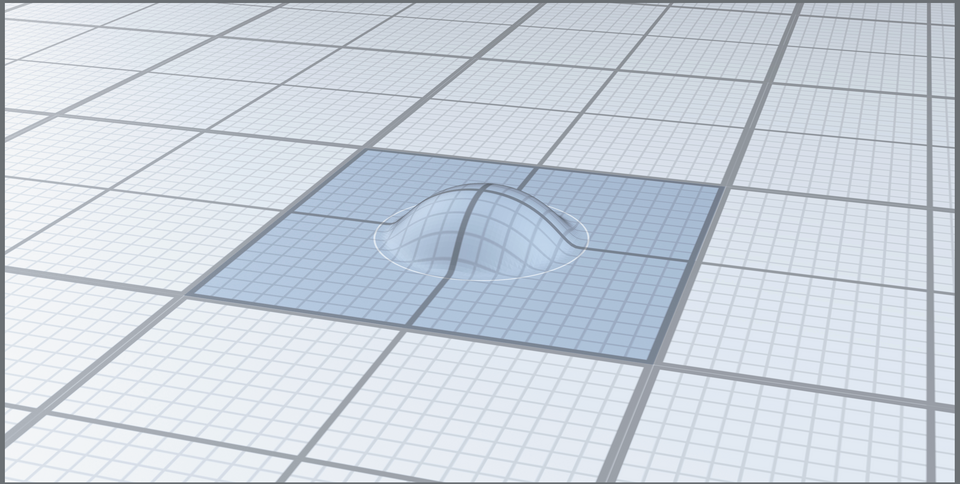
\includegraphics[scale=.8]{images/Bump.png}
\caption{by JoshDif, Wikimedia Commons, licensed under CC BY-SA 4.0}
\end{figure}
\subsection*{Exercício \theexer}
\end{frame}



\subsection*{Partição da Unidade}
\begin{frame}{Partição da Unidade}
	\begin{defin}
		Seja $X$ um subconjunto arbitrário do $\R^\dm$. Dizemos que uma cobertura aberta $(U_\lambda)_{\lambda\in \Lambda}$ de $X$ é \dt{localmente finita} se todo $x\in X$ possui  uma vizinhança $V$ que intercepta apenas um número finito de $U_\lambda$.
	\end{defin}
	
	\begin{prop}[Partição da Unidade, veja {\cite[Theorem 1.2.1]{kesavan}}]
		Seja $\Omega $ um aberto de $\R^\dm$. Dada uma cobertura aberta $(U_\lambda)_{\lambda\in \Lambda}$ de $\Omega$, existe uma família de funções   $(\theta_\lambda)_{\lambda\in \Lambda}$ definidas em $\Omega$, de classe $C^\infty$, chamada \dt{partição da unidade} subordinada à cobertura $(U_\lambda)_{\lambda\in\Lambda}$, tais que
		\begin{multicols}{2}
			\begin{enumerate}
				\item $\supp \theta_\lambda\subset U_\lambda$.
				\item $(\supp \theta _\lambda)_\lambda$ é localmente finita.
				\item $0\leq \theta_\lambda \leq 1$, para todo $\lambda \in \Lambda$.
				\item $\sum_{\lambda\in \Lambda}\theta_\lambda (x)=1$.\\
			\end{enumerate}
			
		\end{multicols}
	\end{prop}
	
\end{frame}

\begin{frame}
\begin{defin}
Sejam \(\Omega\subset \rd\) um aberto, \(K\subset V \subset \Omega\), com \(K\) compacto e \(V\) aberto. Dizemos que \(\phi:\Omega \longrightarrow \R\) é  \dt{uma função corte subordinada a \(V\) e identicamente 1 em $K$.} quando 
\[ \phi\in C_c(\Omega),\ \supp \phi \subset V,\ \phi=1 \text{ em } K \text{ e }
 0\leq \phi(x)\leq 1, \forall\, x\in \Omega.\]
\textbf{Notação do Rudin:}
\[K\prec \phi \prec V\]
%\begin{enumerate}
%\item \(K \prec \phi\)\ significa que \(K\subset \Omega\) é um compacto, \(0\leq \phi(x)\leq 1\) para todo \(x\in \Omega\), \(\phi=1\) em \(K\) e \(\phi\in C_c(\Omega)\).
%\item \(\phi \prec V\)\ significa que \(V\subset \Omega\) é um aberto, \(0\leq \phi(x)\leq 1\) e para todo \(x\in \Omega\),  \(\phi\in C_c(\Omega)\) e \(\supp \phi \subset V\).
%\item \(K\prec \phi \prec V\) quando valem os itens {\itemnum{1}} e {\itemnum{2}}. Neste caso \(\phi\)
%\end{enumerate} 
\end{defin}

\end{frame}

%%%%%%%%%%%%%%%%%%%%%%%%%%%%%%%%%%%%%%%%%%%%%%%%%%%%%%%%%%%%
\begin{frame}

\begin{corol}\label{cut-off}
Seja $K$ um compacto de $\R^\dm$. Então existem \(V\) e \(\phi\in C^\infty_c(\rd)\) tal que
\(K\prec \phi \prec V\).
\end{corol}
	\begin{proof}
		Basta considerar a partição de unidade subordinada à cobertura $(V,\R^\dm\setminus K)$, onde $V$ é um aberto limitado contendo $K$.
	\end{proof}

%\begin{exer}
%	Mostre que existe $\zeta\in C^\infty(\R^\dm)$ tal que $\zeta\equiv 1$ em $B(0,1)$ e $\supp \zeta \subset B(0,2)$.
%\end{exer}
%\subsection*{Exercício \theexer}
\end{frame}





%%%%%%%%%%%%%%%%%%%%%%%%%%%%%%%%%%%%%%%%%%%%%%%%%%%%%%%%%%
\begin{frame}{Suporte em $L^p(\Omega)$}
	\begin{defin}
Seja $u\in L^p(\Omega)$. Definimos o \dt{suporte de $u$}, denotado por {\color{blue}$\supp u$}, como o conjunto obtido pela interseção de todos os subconjuntos fechados de $\Omega$ fora dos quais {\color{blue}$u$} se anula quase sempre.
	\end{defin}

\begin{exer}
Se $u\in C^0(\Omega)\cap L^p(\Omega)$, então as duas noções de suporte coincidem. 
\subsection*{Exercício \theexer}
\end{exer}

\begin{prop}[veja {\cite[Theorem 4.12]{brezis}}]
	O espaço $C_c(\R^\dm)$ é denso em $L^p(\rd)$, para todo $1\leq p<\infty$.
\end{prop}
\end{frame}



